\documentclass{beamer}


% Beamer settings
\usecolortheme{rose}
\beamertemplatenavigationsymbolsempty
\setbeamertemplate{footline}[frame number]

% Packages
\usepackage{amsmath}

\usepackage{pgfplots}
\usepgfplotslibrary{fillbetween}

\usepackage{minted}
\usepackage[T1]{fontenc} % Required by minted to ensure dollar signs are produced instead of pound (sterling) signs

\usepackage{multicol}

\usepackage{booktabs}


\title{OpenMP for Computational Scientists}

\begin{document}

\frame{\titlepage}

%-------------------------------------------------------------------------------
\section{Outline}
\begin{frame}
\frametitle{Course Outline}
Organised as 6 sessions teaching OpenMP plus top-tips for getting good performance.
\begin{enumerate}
  \item OpenMP overview
  \item Data sharing and reductions
  \item Code optimisations
  \item Vectoriation, NUMA and MPI interop
  \item GPU programming with OpenMP
  \item Tasks and Tools
\end{enumerate}
\end{frame}

%-------------------------------------------------------------------------------
\begin{frame}
\frametitle{Thanks}
Thanks go to the following authors, whos own OpenMP tutorials have inspired this one:
\begin{itemize}
  \item Tim Mattson (Intel)
  \item Simon McIntosh-Smith and the HPC team (UoBristol)
  \item Gethin Willians (UoBristol)
  \item and many others
\end{itemize}
\end{frame}

%-------------------------------------------------------------------------------
\begin{frame}
\frametitle{Exercises}
\begin{itemize}
\item This is a hands-on course!
\item Exercises will be set for you to try programming OpenMP yourselves.
\item Sample solutions also provided.
\item All the exercises will be in Fortran.
\end{itemize}

Download code (and slides) from:
\url{https://github.com/UoB-HPC/openmp-for-cs}
\end{frame}

%-------------------------------------------------------------------------------
\begin{frame}
\frametitle{What is OpenMP?}

A collection of compiler directives, library routines, and environment variables for parallelism for shared memory parallel programs.

\begin{itemize}
  \item Create and manage parallel programs while permitting portability.
  \item User-directed parallelization.
\end{itemize}

A \emph{specfication} of annotations you can make to your program in order to make it parallel.

\end{frame}

%-------------------------------------------------------------------------------
\begin{frame}[fragile]
\frametitle{Syntax}
\begin{itemize}
\item OpenMP mostly formed of \emph{compiler directives}\\
  \begin{minted}{fortran}
  !$omp construct [clause [clause]...]
  \end{minted}
  These tell the compiler to insert some extra code on your behalf.

\item Compiler directives usually apply to a \emph{structured block} of statements.
Limited scoping in Fortran means often need \emph{end} directives.
  \begin{minted}{fortran}
  !$omp construct
  ... ! lines of Fortran code
  !$omp end construct
  \end{minted}

\item Library API calls
  \begin{minted}{fortran}
  use omp_lib
  call omp_...()
  \end{minted}

\end{itemize}
\end{frame}

%-------------------------------------------------------------------------------
\begin{frame}[fragile]
\frametitle{Building with OpenMP}

Turn on OpenMP in the compiler:
\begin{minted}{bash}
gfortran *.f90 -fopenmp # GNU
ifort *.f90 -qopenmp    # Intel
ftn *.f90               # Cray (on by default)
pgf90 *.f90 -mp         # PGI
\end{minted}

To also use the API calls within the code, use the library:
\begin{minted}{fortran}
USE omp_lib
\end{minted}

\begin{alertblock}{Note}
No need to include the library if only using the compiler directives.
The library only gets you the API calls.
\end{alertblock}
\end{frame}

%-------------------------------------------------------------------------------
\begin{frame}
\frametitle{Shared memory}
OpenMP is for shared memory programming: all threads have access to a shared address space.

A typical HPC node consisting of 2 multi-core CPUs.
\begin{center}
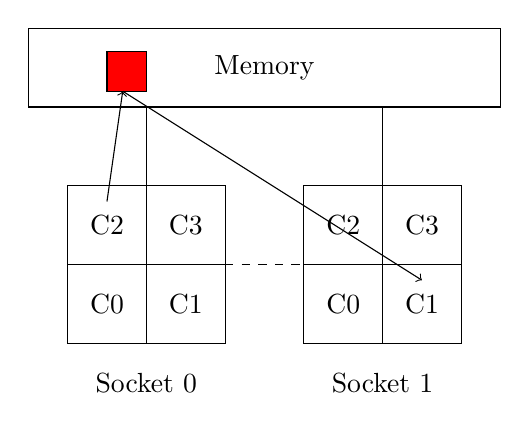
\begin{tikzpicture}
  % Draw 4 cores for socket 0
  \draw (0,0) rectangle (1,1);
  \draw (0.5,0.5) node {C0};
  \draw (1,0) rectangle (2,1);
  \draw (1.5,0.5) node {C1};
  \draw (0,1) rectangle (1,2);
  \draw (0.5,1.5) node {C2};
  \draw (1,1) rectangle (2,2);
  \draw (1.5,1.5) node {C3};
  \draw (1,-0.5) node {Socket 0};

  % Draw 4 cores for socket 1
  \draw (3,0) rectangle (4,1);
  \draw (3.5,0.5) node {C0};
  \draw (4,0) rectangle (5,1);
  \draw (4.5,0.5) node {C1};
  \draw (3,1) rectangle (4,2);
  \draw (3.5,1.5) node {C2};
  \draw (4,1) rectangle (5,2);
  \draw (4.5,1.5) node {C3};
  \draw (4,-0.5) node {Socket 1};

  % Draw large memory
  \draw (-0.5,3) rectangle (5.5,4);
  \draw (2.5,3.5) node {Memory};

  % Connect sockets to memory
  \draw (1,2) -- (1,3);
  \draw (4,2) -- (4,3);
  \draw[dashed] (2,1) -- (3,1); % QPI

  % Show memory shared
  \pause
  \draw[fill=red] (0.5,3.2) rectangle (1,3.7);
  \draw[->] (0.5,1.8) -- (0.7,3.2);
  \draw[->] (0.7,3.2) -- (4.5,0.8);

\end{tikzpicture}
\end{center}
\emph{All} threads (running on a core) access the same memory.

Different to MPI, where processes cannot see memory of another without explicit communication.

\end{frame}

%-------------------------------------------------------------------------------
\begin{frame}
\frametitle{Fork-join model}
Fork join
nested parallel region
\end{frame}

%-------------------------------------------------------------------------------
\begin{frame}
\frametitle{Creating OpenMP threads}
parallel region
talk about synch at end of region
\end{frame}

%-------------------------------------------------------------------------------
\begin{frame}
\frametitle{Pthreads}
Show the same in Pthreads
Thread pool
\end{frame}


%-------------------------------------------------------------------------------
\begin{frame}
\frametitle{Environment variables}
Setting number of threads via env variables, API and clause
\end{frame}

%-------------------------------------------------------------------------------
\begin{frame}
\frametitle{Vector add}
Vector add with SPMD (no worksharing)
\end{frame}

%-------------------------------------------------------------------------------
\begin{frame}
\frametitle{Synchronisation}
Critical, atomic, barier, ordered, flush, locks
\end{frame}

%-------------------------------------------------------------------------------
\begin{frame}
\frametitle{Worksharing}
parallel for vadd

\end{frame}

%-------------------------------------------------------------------------------
\begin{frame}
\frametitle{Scheduling}
schedule clause

\end{frame}

%-------------------------------------------------------------------------------
\begin{frame}
\frametitle{Nested loops}
Collapse
Mention issues with SIMD/alignment?

\end{frame}

%-------------------------------------------------------------------------------
\begin{frame}
\frametitle{5-point stencil example}
Do parallelism of a structured grid 5-point stencil
\end{frame}

%-------------------------------------------------------------------------------
\begin{frame}
\frametitle{nowait clause}
nowait
\end{frame}

%-------------------------------------------------------------------------------
\begin{frame}
\frametitle{Sections}
sections, single, tasks?
\end{frame}

%-------------------------------------------------------------------------------
\begin{frame}
\frametitle{Nested threads}
sections, single, tasks?
\end{frame}

%-------------------------------------------------------------------------------
\begin{frame}
\frametitle{Resources}
OpenMP secficiation (not for the faint hearted)
Online tutorials
Books
\end{frame}

%-------------------------------------------------------------------------------

\end{document}
